\documentclass{article}
\usepackage[utf8]{inputenc}
\usepackage{listings}
\usepackage{graphicx}
\usepackage{float}
\begin{document}
\author{Harry Hughes}
\date{5-24-2017}
\title{Dare Technical Report}
\maketitle
\begin{abstract}
This paper describes the DARE tracer, the most recent deliverable of the DARE project. This tracer is developed exclusively for use with PLASMA, but the design principles used in the tracer can be applied for any library. It utilizes a new approach to program profiling and obtains timing information at the subroutine level. Future work includes adding new modules that expand the tracer project to a discrete-event simulator.

\end{abstract}

\section{DARE Project Overall Objective}
\paragraph{}
The rapid and ongoing revolution in processor design has substantially exacerbated the longstanding problem
of tuning the performance of a parallel program intended to execute on a given system. Although experience
shows conclusively that the wrong choice of parameters like task-granularity and task-binding can lead
to severe performance penalties, the extreme complexity of what is actually happening when a parallel
application executes on scalable hybrid systems makes it nearly impossible, based only on prior knowledge
of the program and a description of the architecture, to ascertain the best tuning parameters in advance. 
\paragraph{}
For
example, the optimum task-granularity is heavily dependent on the problem size, and the results obtained
for smaller problems running on fewer cores do not extrapolate to larger problems running on more cores.
Additionally, accurately tuning and modeling the performance on a large number of cores requires large input
sizes, which quickly becomes prohibitively expensive. In the Data-driven Autotuning for Runtime Execution
(DARE) project, we aim to discover a solution to this problem by building on empirical techniques that we
have helped to pioneer in the field of numerical libraries

\section{What is PLASMA}
\paragraph{}
The Parallel Linear Algebra Software for Multicore Architectures (PLASMA) package is a dense linear algebra package at the forefront of multicore computing, designed to deliver the highest possible performance from a system with multiple sockets of multicore processors. PLASMA achieves this objective by combining state-of-the-art solutions in parallel algorithms, scheduling, and software engineering. Currently, PLASMA offers a collection of routines for solving linear systems of equations, least square problems, eigenvalue problems, and singular value problems.
\paragraph{}
PLASMA relies on runtime scheduling of parallel tasks, which is based on the idea of assigning work to cores based on the availability of data for processing at any given point in time. The concept, which is sometimes called data-driven scheduling, is closely related to the idea of expressing computation through a task graph, often referred to as the DAG (Directed Acyclic Graph), and the flexibility of exploring the DAG at runtime.

\section{What is core\_blas}
\paragraph{}
The parallel tasks that PLASMA schedules to run on cores come from a collection of subroutines collectively referred to as core\_blas. These subroutines are single threaded and carry out some matrix operation. Core\_blas functions are wrappers for library functions such as MKL.

\section{Motivation}

\paragraph{}
As described above, the PLASMA library carries out large matrix operations by partitioning them into many smaller BLAS subproblems solvable by a single subroutine on a single thread. These subroutines can be thought of as the building blocks of the solution. They are typically implemented in a vendor library such as Intel's MKL. Optimizing PLASMA or any library like it requires the developer to be able to identify bottlenecks when it is run in real-life scenarios. The subroutines described above represent the ideal observable units of granularity from the standpoint of a developer. A tool that affords developers with runtime scheduling patterns and runtime timing information in terms of these units as discrete events would be very useful for optimization purposes.
\paragraph{}
Many conventional tracers provide the functionality to trace program execution as subroutines as discrete events. Most of these tracers are designed for the general case; they can provide tracing information for any arbitrary user program. This flexibility comes at a great cost when compared to a tracer that is designed for a particular platform only. 
\paragraph{}
Conventional profiling tools typically rely on code instrumentation to obtain tracing information. This likely requires recompilation in addition to incurring additional overhead. They are also inflexible in the sense that developers cannot integrate their own profiling related modules into them. Profiling tools such as these are designed with no prior knowledge or assumptions about the applications they will be tracing. Thus, their design makes sense. However, a lighter-weight and more flexible solution is possible.

\section{Implementation}
\paragraph{}
%Describe function hooking
The DARE Tracer uses a novel design strategy and is designed to work specifically with PLASMA. The fundamental concept of operation is quite simple. When a user application calls routines from the PLASMA library, those routines in turn call core\_blas functions. In PLASMA's software implementation, these functions are defined as weakly linked symbols. Thus, if they are strongly defined elsewhere, the strong definition will be used and the weak one ignored.
\paragraph{}
The DARE Tracer redefines each weak core\_blas symbol according to the following pseudocode:

\begin{lstlisting}[language=C]
/* parameters list left empty for brevity */
void core_function(...)
{
    wrapper_above(...);
    
    (*original_core_function)(...);
    
    wrapper_below(...);
    
    return;
}
\end{lstlisting}

Each function to be traced is replaced by an instrumented version of itself defined in the DARE Tracer source code. 

\paragraph{}
The DARE Tracer build system automatically generates code like that shown above for each function defined in core\_blas. This task is carried out by a python script that scans core\_blas header files and extracts every function declaration with the format of a core\_blas function. Definitions for the functions denoted ``wrapper\_above'' and ``wrapper\_below'' may be supplied to the build system by the developer. This makes the system very customizable.

\paragraph{}
For the DARE Tracer to function according to the description above, the following conditions must be met:
\begin{enumerate}
\item{} PLASMA and core\_blas must be compiled as shared object libraries. (So weakly linked core\_blas functions can be overridden by the tracer at runtime)
\item{} Your compiler must support weak symbol linkage. (This is so that the core\_blas functions can be overridden with their instrumented versions)
\item{} You must have Python. (The build system relies heavily on Python)
\item{} You must have CMake. (The build system relies on CMake)
\end{enumerate}


\section{Usage}
\subsection{Configuration}
The tracer must be configured before the first use. This can be done by running a file called ``autogen.py'' located in the top-level project folder. This script takes a single command line argument, an XML configuration file. This file must contain the following:

%Captain! Remove the defunct command line arguments section later
%Captain! Make sure to note the fact that the wrap.xml file comes prepackaged
%To run the default cases.
\begin{enumerate}
\item{} --help/-h: Prints help message. (Optional)
\item{} --dir/-d: Full path to top level PLASMA directory. (Required)
\item{} --wrapper/-w: The tracer's XML configuration file. (Required)
\item{} --include/-i: Space-separated list of paths to the directories containing the header files for the tracing wrappers. (Optional)
\item{} --trace\_h/-r: Space-separated list of the header files declaring the tracing wrappers. (Optional)
\item{} --trace\_c/-c: Space-separated list of .c or .cpp files defining the tracing wrappers. (Optional)
\end{enumerate}

The project is configured via options specified as XML tags in an XML configuration file. It must follow the format of the one shown below:
%Show code listing
\begin{lstlisting}[language=XML]
<config>

    <wrap_above_func> 
        <name> trace_cpu_start </name>
        <file_extension> .c </file_extension>
        <declaration> void trace_cpu_start() </declaration>
    </wrap_above_func>
    
    <wrap_below_func> 
        <name> trace_cpu_stop </name>
        <args>
            <arg configurable = 'True' string = 'True'> color_list </arg>
        </args>
        <file_extension> .c </file_extension>
        <declaration> void trace_cpu_stop(const char *) </declaration>
    </wrap_below_func>

    <use_default kernel_colors = 'color_list'> 1 </use_default>

    <color_list>
        <pair> <key> default </key> <value> "0xEE82EE" </value> </pair>
        <pair> <key> core_dgemm </key> <value> "0x00FFFF" </value> </pair>
        <pair> <key> core_dsyrk </key> <value> "0xFFC0CB" </value> </pair>
    </color_list>

    <plasma_dir> /Users/hhughe11/research/plasma </plasma_dir>

    <include_dirs>
    <dir> /Users/hhughe11/research/plasma/include </dir>
    <dir> /Users/hhughe11/research </dir>
    </include_dirs>

    <trace_h>
    <h> /Users/hhughe11/research/plasma_trace.h </h>
    </trace_h>

    <trace_c>
    <c> /Users/hhughe11/research/trace.c </c>
    </trace_c>
    
</config>
\end{lstlisting}

Each tag in this example will be briefly described below:
\subsection{config}
All configuration tags must be nested under ``config''.

\subsection{$<$wrap\_above\_func$>$}
\begin{itemize}
\item $<$name$>$ The name of the function without any parentheses or parameters. This option is ignored if the default wrappers are used.
\item $<$file\_extension$>$ This can be either ``.c'' or ``.cpp'' to indicate whether the function is defined in a C or CPP file. This option is ignored if the default wrappers are used.
\item $<$declaration$>$ This is the declaration of the function as it appears in source code. Note that no semicolon is included.
\end{itemize}
\subsection{$<$wrap\_below\_func$>$}
\begin{itemize}
\item $<$name$>$ The name of the function without any parentheses or arguments.
\item $<$args$>$ Each function parameter is described with this tag. If the argument is a character string, the ``string'' attribute is accordingly set to ``True''. If the value of the argument depends on which core\_blas kernel it is being called inside, the ``configurable'' attribute must also be set to ``True''. The value of the tag denotes another tag in the XML file that contains the mappings from core\_blas kernel to color. The tag must contain key-value pairs as shown. In this case ``color\_list'' is the name of the mapping.
\item $<$file\_extension$>$ As before, this option indicates the extension of the file where the function is defined.
\item $<$declaration$>$ As before, this is the declaration of the function as it appears in source code with no semicolon.
\end{itemize}
\subsection{$<$use\_default$>$} This option indicates whether the DARE Tracer should use the default function wrappers or use the functions supplied by the user. A value of `1' indicates that the default wrappers should be used while `0' indicates otherwise. The ``kernel\_colors'' attribute of this tag indicate the core\_blas kernel to color mapping to be used with the default wrappers. In this example, the default case uses the same colors as the custom wrappers.
\subsection{$<$plasma\_dir$>$} This indicates the full filepath of the top-level PLASMA directory.

\subsection{$<$include\_dirs$>$} This tag contains the full paths to all the directories that contain any header files for the user-defined wrapper functions.
\begin{itemize}
\item $<$dir$>$ Each full filepath of a directory is contained in a ``dir'' tag.
\end{itemize}
\subsection{$<$trace\_h$>$} This tag contains all header files needed by the tracing wrappers if the tracer is to be configures with user-defined wrappers.
\begin{itemize}
\item $<$h$>$ Full filepath to header file. Each header file gets its own pair of ``h'' tags.
\end{itemize}
\subsection{$<$trace\_c$>$} This is the same as the ``trace\_h'' tag but with .c or .cpp files.
\begin{itemize}
\item $<$c$>$ One file per tag pair.
\end{itemize}
\subsection{Final Build}
\paragraph{}
Once all options in the configuration file are satisfactory, the tracer can be generated as a dynamic library simply. The ``autogen.py'' script located in the top level project directory must be run as: 

\begin{lstlisting}[language=bash]
python autogen.py wrap.xml
\end{lstlisting}

This is assuming that the XML configuration file is called ``wrap.xml'', but it can be named anything.

\subsection{Tracing an Application}
%illustrate the flexibility of the system.
\paragraph{}
The tracing workflow will be delineated by example. Assume that the user wishes to trace the following application, main.c. This program does not do anything useful; it is simply to illustrate the usage of the tracing library. It creates two triangular matrices of a specified size, multiplies them with plasma\_dgemm, and then decomposes them with a Cholesky factorization with plasma\_dpotrf:

\begin{lstlisting}[language=C]
#include "plasma.h"
#include "stdio.h"
#include "stdlib.h"
#include "sys/mman.h"
#include "fcntl.h"

void gen(double *matrix, int n)
{
    int i;
    int j;

    srand(time(NULL));

    for(i = 0; i < n; i++)
    {
        for(j = 0; j < n; j++)
        {
            matrix[j*n+i] = (double)((rand()%256)+1);
        }
    }

    return;
}

int main (int argc, char *argv[]) 
{
  int tid;
  int n;
  double *a;
  double *b;
  double *c;
  int len_bytes;

  printf("enter n: ");
  scanf("%d", &n);
  len_bytes = n*n*sizeof(double);

  /* create a new buffer for the result  */
  a = (double *)malloc(len_bytes);
  gen(a, n);
  
  c = (double *)malloc(len_bytes);
  
  plasma_init();

  /*Multiply two triangular matrices*/
  plasma_dgemm
  (
   PlasmaNoTrans 
  ,PlasmaTrans
  ,n
  ,n
  ,n
  ,1.0
  ,a 
  ,n
  ,a
  ,n
  ,0.0
  ,c
  ,n
  );

  /*Decompose the product with a Cholesky factorization*/
  int r = plasma_dpotrf
  (
   PlasmaUpper
  ,n
  ,c
  ,n
  );

  plasma_finalize();

  free(a);
  free(b);
  free(c);

  /* check the return value */
  printf("Cholesky returned %d\n", r);

  return 0;
}
\end{lstlisting}

Not regarding the various compiler options necessary to point the linker to the correct include directories, the command line compilation string for this program looks something like this:
\begin{lstlisting}[language=bash]
gcc main.c -o main -lplasma -lcoreblas
\end{lstlisting}

To use the tracing library to produce trace output, the previously described invocation must simply be changed to:
\begin{lstlisting}[language=bash]
gcc main.c -o main -lplasma -lcoreblas -ltrace_lib
\end{lstlisting}
Where ``libtrace\_lib.so'' is the output of the tracer configuration described above. If the XML configuration file specifies that the default wrapper functions are to be used, the output of the program invocation is a file called ``kernel\_data.txt''. Located in the top-level PLASMA directory is a file called ``plot.py''. Simply run this program in the same directory as ``kernel\_data.txt'' and it plots the contents as a Gantt chart. A portion of the trace output of the ``main.c'' program shown above is shown in figure 1:
\begin{figure}[H]
\caption{Kernel Durations throughout time}
\begin{center}
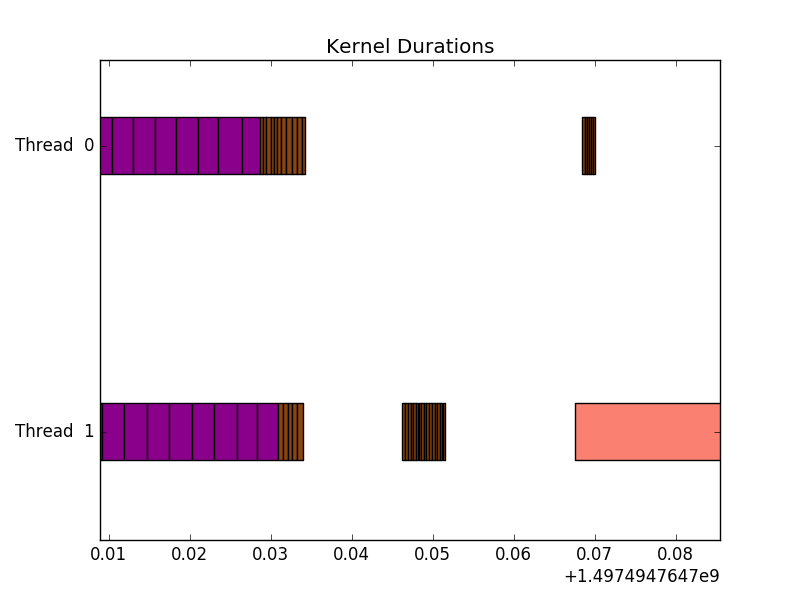
\includegraphics[scale=0.75]{figure_1.png}
\end{center}
\end{figure}
The colors represent the kernels indicated in the legend, as shown in figure 2:
\begin{figure}[H]
\caption{Kernel to color legend}
\begin{center}
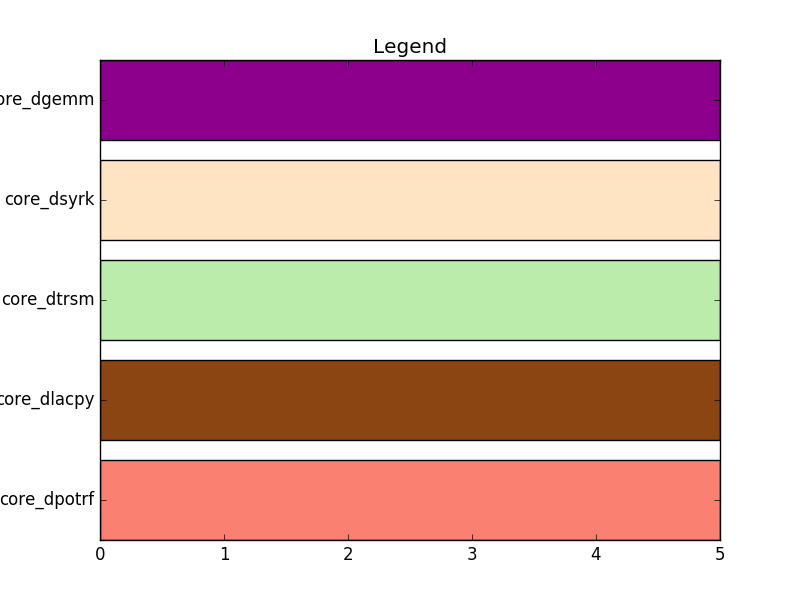
\includegraphics[scale=0.75]{figure_2.png}
\end{center}
\end{figure}
An example of custom tracing output 

\section{Future Work}
\paragraph{}
A major design goal of the DARE project is extensibility through modularity. Thus, more interchangeable tracing modules need to be developed. In addition, a new discrete event simulation module will also be developed. This will produce virtual tracing output in a fraction of the time it would take to produce real output. This will be an invaluable tool for developers researching large problems on extensive heterogeneous architectures. Developing an accurate simulator introduces a slew of non-trivial problems that must be overcome.
\end{document}











